\chapter{State of the Art}
\label{ch:stateoftheart_report}

\section{Literature Review}
\label{ch:literaturereview_report}

In order to tackle the research questions, different disciplines of software engineering such as Complex datasets, Compiler reporting, Continuous integration, Refactoring tools, Issue tracker, Stack Overflow, Gamification, Usability Engineering are looked into and studied what ideas we can adapt into our scenario along with own novel solution ideas. \\ \\

After doing the literature review in the disciplines mentioned above, there are a few essential takeaways in the scope of this thesis. In the area of ‘Complex datasets’, Dix et al. \cite{Dix} with their current research talks about more complex grouping and linking of datasets in the context of a user interface of Spreadsheets application. There could be two datasets with fields having a similar meaning and fields that are entirely different. So, the key takeaway is about design lessons of extensibility of columns. For example, ‘venues were geocoded to allow spatial graphs’ could be related as dates in bug reports to some standard format. It is done for all tools used and then shown on a unified interface. Next, Gaur et al. \cite{Gaur} speaks about the linear search problem in indexing as it takes more time for large volumes of data. So, different parameters are introduced to decrease computation time. For example, it linearly searches a database with toys.  It takes more time than a modified query like ‘a toy in red colour and horse types’.  By looking at two parameters, i.e., colour and type simplifies the search. This analogy sparks the idea of grouping bugs as per module, bug type, which could ease user in finding a particular bug on an interface. \\ \\

In the area of ‘Compiler reporting’, Horning et al. \cite{horning} mentions the importance of error logging with statistics as to what the compilers are expected to tell the user. It also mentions the importance of stating what kind of bugs does the tool did not find along with bugs found, but in reality, this questions the scalability. So, the key takeaway is that it is ideal for showing the number of specific bugs founds in an analysis. Next in the area of ‘Refactoring tools’, Dustinca \cite{dustinca} talks about how these tools are to be built and in user context, it has to overcome the barrier of discoverability which means the difficulty of use. To assist the developer on this issue, they introduced a smart tag in the context of the user editor and notified which parts of the code we can refactor. This analogy emphasises the importance of ‘on-board’ phase, which plays a vital role in the gamification \cite{gamify} discipline. Hayashi et al. \cite{Hayashi} illustrate the importance of task-level commits in order to maintain an edit history of refactoring. This concept gives an idea of which a user does a bug-fix level commit to addressing the traceability scenario. Mealy et al. \cite{Mealy} mentions about the importance of usability for software refactoring tools, and this could perhaps give some basic guidelines similar to knowing Usability Engineering \cite{usability} discipline. \\ \\

In the area of ‘Issue tracker’, Baysal et al. \cite{Baysal} mentions reducing the information overload for a developer in using the issue tracker. It is found out in their research paper that there is too much of information they receive. It confuses the developer in how to react, for example, the developer receives a high number of bugs reported via email, and this leads to a situation where the developer ignore the email. They found some exciting solution ideas, such as having a private dashboard for each developer as it becomes easy to react to issues corresponding to them. Expressiveness is one other mentioned in their paper, which says an example, severity or priority are vague terms to describe a bug. Perhaps it is ideal to describe the priory as per team decision instead of personal choice. This approach signifies in categorising the results as per categories in our unified interface. Next in ‘Stack Overflow’, in a research paper by Wang et al. \cite{stack} it is found there are 10934198 questions on a ‘User Interface’ topic, for example. It is quite challenging to go through such a high volume database. However, the Stack Overflow team has a friendly user interface, as shown in the following \autoref{fig:stackoverflow}. It uses some clean filter techniques such as tags for each topic, priority and trending. A research by Treude et al. \cite{Treude.2011} found out that most of the questions (72.30\%) in Stack Overflow have between 2 and 4 tags. This approach could perhaps ease in filtering/indexing issues. \\ \\

\begin{figure}[hbt!]
	\centering
	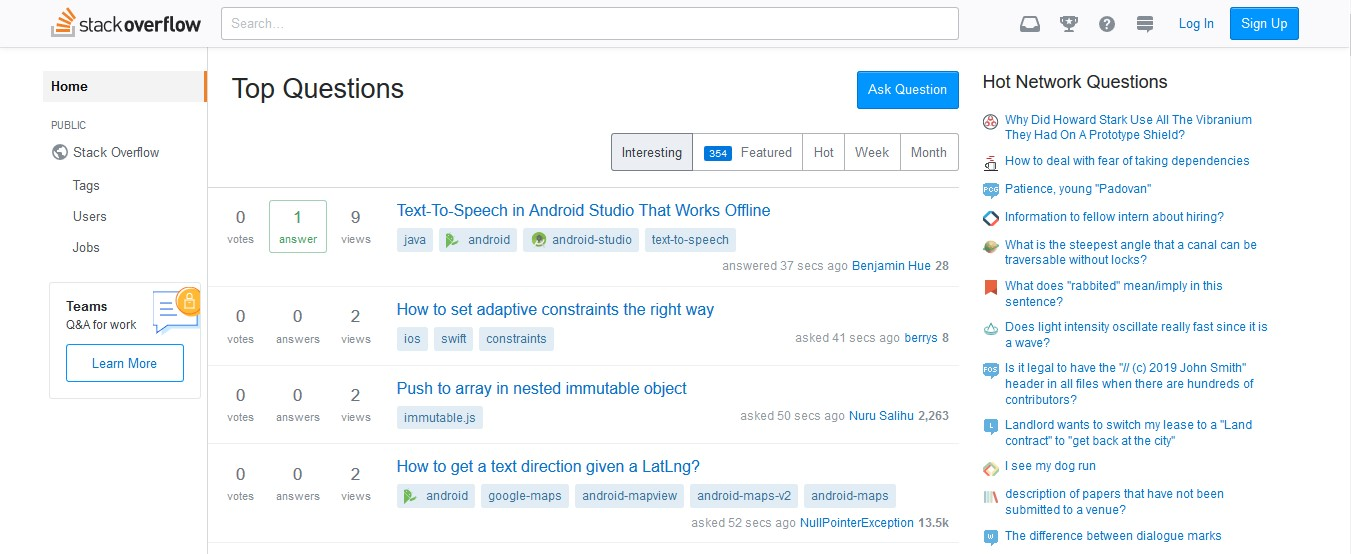
\includegraphics[width=\linewidth]{figures/stackoverflow}
	\caption{An user interface of Stack Overflow Website. \cite{stackoverflow}}
	\label{fig:stackoverflow}
\end{figure}

\section{Motivation}
\label{ch:motivation_report}

Static analysis plays a prominent role in releasing bug-free software. Despite that, essential tools suffer from well-documented usability issues. \cite{CB16,JSMB13} Johnson et al. \cite{JSMB13} found design flaws in current static analysis tools and the need for an interactive mechanism in assisting developers in fixing bugs. They interviewed with 20 participants, of which 16 are professional developers, and 4 are graduate students. The exciting findings are if the output of static analysis tool is user-friendly and intuitive, false positives and high number of warnings could be less problematic for a developer. Also, showing call hierarchies with which parts of code are affected by a bug, and be able to share settings with pre-defined coding standards among the team. Next, need of a web browser for reacting on the analysis output, for instance, adding a comment to a bug which goes out of context to the developer. Christakis et al. \cite{CB16} also did an empirical study on what developers want and need from program analysis. They surveyed by sending invitations to 2,000 developers within their organisation, i.e., Microsoft and received 375 responses. The resultant data is analysed and found that there are some obstacles which hinder the usage of a static analysis tool by a developer such as ‘Wrong checks are on by default’, ‘Too many false positives’, ‘Too slow’, ‘Complex user interface’. Being a user interface an obstacle for a developer along with other usability problems is noteworthy. The key takes away from the papers, as mentioned earlier, is the importance of usability in the on-going adaption of static analysis tools. \\

In general, the setup of most of the recent research \cite{CB16} \cite{JSMB13} done in the area of Static Code Analysis is like assuming a single project in an organisation. Further, they assume a single person is working on a single project with a single tool tackling a single type of problems. Somehow, the assumptions are made singular to address a specific issue in their research. However, in practice, i.e., in the real world of software engineering, numerous people are working in teams for multiple projects at a time. Each project uses multiple tools in their software development. Even in the case of Static Code Analysis, multiple tools are used, which are each capable of addressing several types of issues in order to find more code flaws. \cite{SCALe} \\

Habib et al. \cite{habib} did a study on static bug detectors about how the tools find many of the bugs. They found that tools used for their research are complementing each other in some bug findings.  Thereby, expressed opinion that developers might want to combine the tools and so researchers could address how to reconcile the bug findings reported by multiple tools. This open challenge gives additional motivation for this thesis work.

\section{Related Work}
\label{ch:relatedwork_report}

\subsection{Current Research in Using Multiple Analysis Tools}

In the current research, we could see the usage of multiple tools in the software industry, where each tool is different in computation approaches. One could be standard run on nightly builds, for example, with Checkmarx \cite{checkmarx} tool or could be following incremental analysis, which means only testing the changed version of code instead of running analysis on complete codebase. The reasons for using multiple tools could be as each tool is capable of detecting bugs with different coverage, \cite{bessey2010few} \cite{delaitre2015evaluating} it could help in finding more bugs easily which are not found by tool but the other. \cite{plakosh2014improving} There is also research \cite{flynn2018prioritizing} going in the direction of using multiple static analysis tools in order to prioritise the bug warning alerts. There is a paper \cite{meng2008approach} published in 2008 which uses results of three different static analysis tools for a programming language, Java and merges them in order to show warnings to the developer. \\ \\

Sadowski et al. and team developed a framework called Tricorder \cite{tricorder} which mentions about using multiple tools where each tool covers separate bug coverage. The results are displayed during the code review and published by a bot called ReviewBot. They evaluated with a summative approach using click rates by the user, which shows which tool is better in comparison to others. Tricorder is closed source for Google infrastructure, and so this is specific for Google developers. Later, emerges a new tool which is similar to Tricorder with the philosophy behind it, such as workflow integration, data-driven usability improvements, empower users to contribute were transformed into development of Shipshape \cite{shipshape} which is an open-source static program analysis platform. It allows custom analysers to plug in through a standard interface. This tool commonly runs as a command-line interface. It has a different architecture to support the needs of open-source projects. However, the Tricorder influences heavily on its API and design. The drawbacks of this tool being it is heavily dependent on docker and not much workflow integration points with no feedback collection. Google developers archived this project because of the lack of active development. Recently, a new tool from Google called Tricium, \cite{tricium} which is also open source and more focussed for Chromium development workflow, i.e., Chrome infrastructure with philosophy or ideas from Tricorder. Tricium supports robot comments like Tricorder does, which is unlike with Shipshape having only command-line interface. \\ \\

Cifuentes et al. and team developed a framework called Parfait \cite{parfait} using multiple tools which address the issues with scalability and precision. For scalability, it checks the easy and expensive analysis for each bug type and for precision it tracks each bug whether it is real, potential or not. \\ \\

Although we have seen the current research trends and their direction, the usability aspect is not addressed so far in the context of using multiple tools. There are no research papers found addressing the usability issue with multiple tools in a single interface. The multiplicity of tools used for a single project and that too with different computation capabilities brings a new challenge. One tool could produce results in no time and others could take more time in comparison. This indifference could lead to a situation of breaking the usability of the user interface. On that challenge, this thesis aims to address such a scenario with a problem statement as “How to integrate the results of multiple static analysis tools in a unified user interface?”. \\ \\

The thesis work begins by brainstorming on the problem statement. As a result, different research questions are brought up. Out of which, we selected three primary questions concerning available sources, scope and limitations of thesis time frame. \\ \\


\subsection{What Current Tools do?}

Let us now examine each research question and see what the current tools behave like in similar scenario. \\ \\

\textbf{1. How to display the results of the same codebase from different analysis tools?} \\

This question needs to address the scalability aspect of displaying results as usage of multiple tools results in redundancy and a high number of warnings with more coverage. The following \autoref{fig:findbugs-results} shows how a FindBugs \cite{findbugs} static analysis tool shows results for a project \cite{findbugs-example}. This kind of display could be the same with other tool, and so when we use multiple tools, there is a need for a better user interface. \\ \\

\begin{figure}[hbt!]
	\centering
	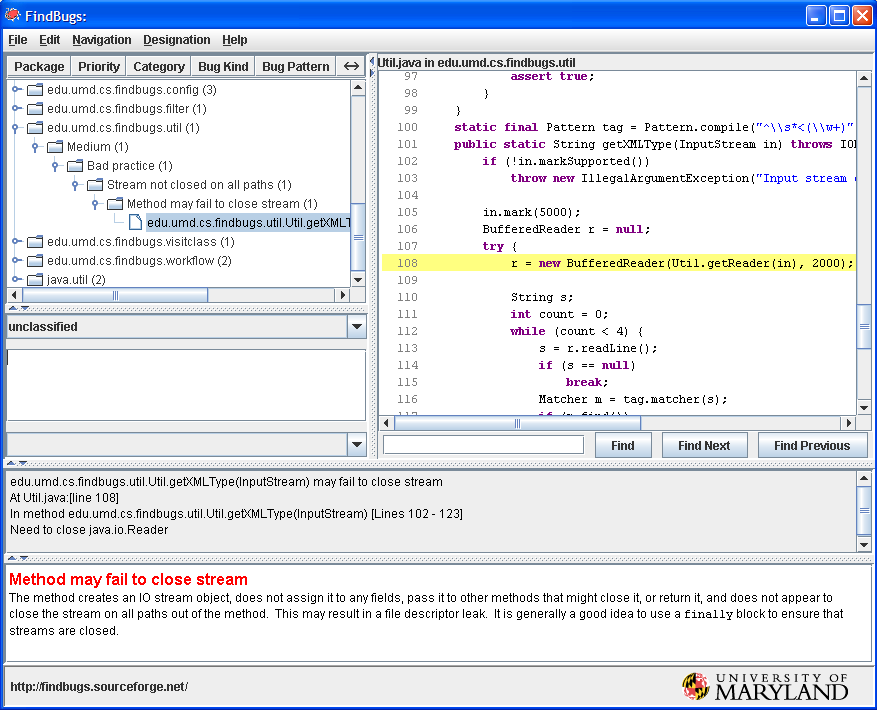
\includegraphics[width=\linewidth]{figures/findbugs-results}
	\caption{A preview of FindBugs scan results.}
	\label{fig:findbugs-results}
\end{figure}


The Tricorder shows the results with multiple tools, as seen in the following \autoref{fig:tricorder-results}, where two findings each from different tool. \\ \\

\begin{figure}[hbt!]
	\centering
	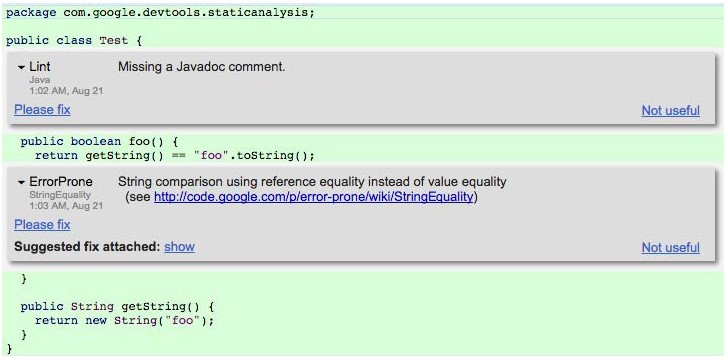
\includegraphics[width=\linewidth]{figures/Tricorder}
	\caption{A preview of Tricorder scan results. \cite{tricorder}}
	\label{fig:tricorder-results}
\end{figure}

\textbf{2. What feedback works to know that bug fixing is on-going?} \\

This question needs to address the scenario where one tool could give an instant update on the bug fixing process, and others might take more time to analyse and report the update on it. In the design aspect, especially the User Interface needs to be adaptive \cite{NB18} enough as static analysis tools sometimes take a long time to stop, and there is no intuitive feedback provided. Also, One exciting aspect of Johnson et al. \cite{JSMB13} study is about the importance of feedback from tools without disrupting the developer workflow. Traditionally, the project files are added to FindBugs \cite{findbugs} tool as seen in the \autoref{fig:findbugs-scan} in order to start the scanning. Then the user has to wait for some minutes to see the results. There was no feedback in the process of scanning. \\ \\

\begin{figure}[hbt!]
	\centering
	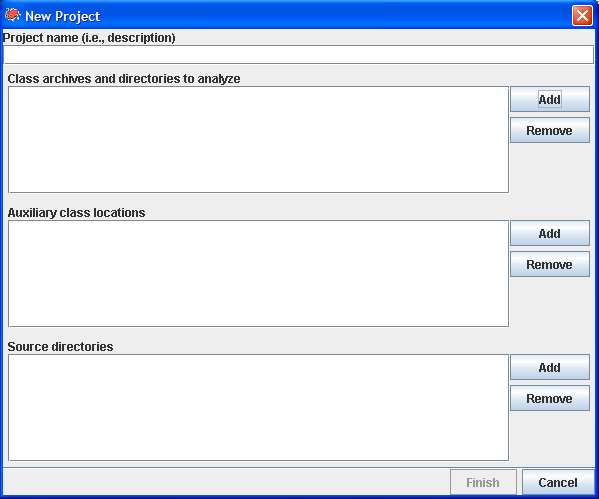
\includegraphics[width=\linewidth]{figures/findbugs-scan}
	\caption{A preview of initiating FindBugs to scan a project. \cite{findbugs}}
	\label{fig:findbugs-scan}
\end{figure}

Back in the history of Computer Science, there is an observation made when the user interface is non-responsive, the user shuts down the system. After that, comes to the implementation of user interface called Ghost screen by Colleran et al. \cite{colleran} who patented the method which manages application programs with non-responsive user interfaces in the year 2005. About the response times, NN Group \cite{nn} states that if the execution of a particular task takes 0.1 up to 1 second, then there is no need for feedback, show the result. If it takes 10 seconds, there should be feedback, and if it is variable every time, then per cent bar \cite{Borman} is essential. However, sometimes, it could be overkill to use as it causes stress to the user by the principle of display inertia. If the time taken by a task is unknown, then there has to be feedback like a spinning ball. If in an example of a task being to scan databases, then it has to report user about what tool scans the database currently. Overall, there has to be feedback stating that the system is working, if not indicating what is doing. This time indifference motivates to know how responsiveness in terms of usability is vital to consider in the development of modern tools. Further, we need to address this in the context of using multiple tools. \\ \\

\textbf{3. How to carry traceability of bug fixing?} \\

In the scenario, where the user has picked a bug to fix and worked on it and later he submitted for analysis. Then the bug could either get fixed or new bugs could have been introduced or different bugs got resolved by fixing the one bug. All these might have taken place, and this is uncertain. Thereby it would be better to have traceability in order to monitor the changes happening in the context of bugs or somehow safeguard the code repository from future bugs. \\ \\

As per the related work in research, \cite{heinemann2014teamscale} a tool named ‘Teamscale’ \cite{teamscale} shows the influence on the quality status for each change in code backed by version control commits. For a change, it shows how many newly added quality problems or the ones removed. Following \autoref{fig:teamscale} illustrates further. \\ \\

\begin{figure}[hbt!]
	\centering
	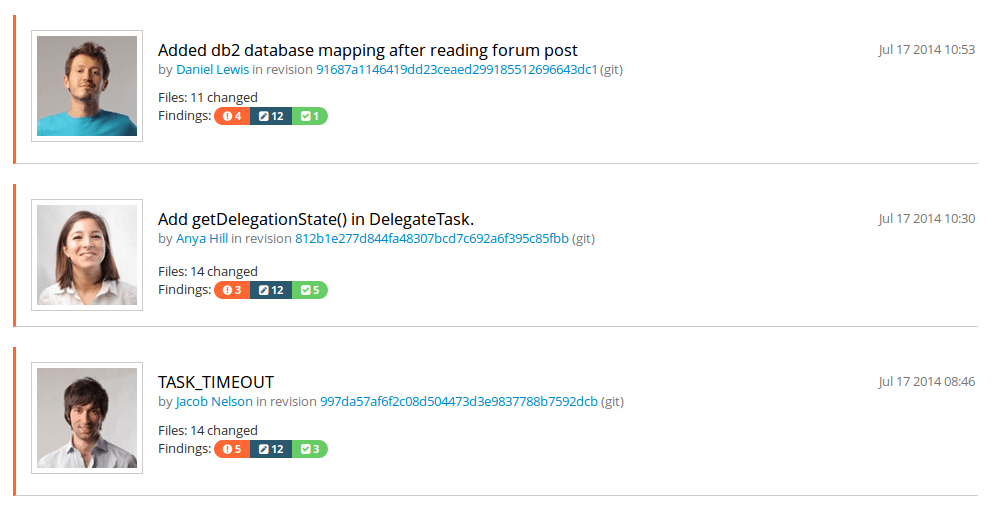
\includegraphics[width=\linewidth]{figures/teamscale}
	\caption{A Teamscale feature of showing quality status with code changes. \cite{teamscale}}
	\label{fig:teamscale}
\end{figure}

\let\cleardoublepage\clearpage

